\newpage
\section{Daten formatieren}
\label{formatdata-main}
Das Anzeigen von Daten in einer View hat zum Ziel, dem Anwender Informationen zu vermitteln. Zu diesem Zweck sollten diese Informationen in einer geeigneten Form präsentiert werden. Diese Form variiert dabei in Abhängigkeit zu den Daten. Beispiele dafür sind die Anzeige von Gleitkommazahlen mit einer begrenzten Anzahl von Nachkommastellen oder Datumswerte, die anhand der landestypischen Eigenschaften am Standort des Anwenders formatiert sind. Beim \gls{mvc}-Konzept von AngularJS könnte diese Formatierung im Controller oder bereits vorher in einem Service stattfinden. Um die jeweiligen Controller und sonstigen JavaScript-Code von solchen Formatierungen zu befreien, ermöglicht AngularJS das Definieren von Filtern. Filter sind JavaScript-Funktionen, die einen Eingangswert in einen Ausgangswert umwandeln und über das \gls{html}-Markup verwendet werden können. Das Prinzip und die Verwendung ähnelt dabei stark dem Mechanismus der \gls{Pipes} unter Linux. Aufgrund dieser generischen Funktionsweise können Filter in vielen Einsatzszenarien verwendet werden. Neben dem Formatieren von numerischen Werten oder Datumsangaben eignen sie sich außerdem dafür, ganze Listen zu sortieren oder zu filtern. Darüber lassen sich komplexe Filterszenarien ohne JavaScript-Implementierung und allein über ein \gls{html}-Markup realisieren. Weitere Szenarien beinhalten das Verkürzen von langen Texten mit einer \glqq Mehr anzeigen\grqq{} Schaltfläche oder eine komplette Internationalisierung durch die Übersetzung von Texten.\cite{AJSFilter}
\\\\
Filtern stellt demnach eine sinnvolle Möglichkeit dar, Daten zu formatieren. Doch welchen Einfluss haben Filter auf die Performance? Dieser Frage soll in diesem Abschnitt nachgegangen werden, indem ihre Auswirkungen auf die Performance analysiert und gemessen werden. Im Anschluss an diese Betrachtung werden Implementierungen vorgestellt, mit denen die Performance generell oder für spezielle Szenarien verbessert werden kann.
\\\\
Technisch gesehen sind Filter einfache JavaScript-Funktionen, die einen Eingabewert und Parameter erhalten und einen Ausgabewert zurückliefern. Der erste Faktor, der die Performance beeinflussen kann, ist die Implementierung dieser Funktion. Filter werden im \emph{\$digest}-Zyklus aufgerufen, wenn sich der Eingangswert geändert hat. Theoretisch haben Filter bei Interaktionen durch den Anwender dadurch keinen negativen Einfluss auf die Performance. Bei gleichbleibenden Eingangswerten werden sie nur einmalig ausgeführt. Dies trifft jedoch nur auf einfache Werte wie Strings oder Zahlen zu. Die Überprüfung, ob sich komplexe Werte wie Objekte oder Arrays geändert haben, ist sehr aufwendig und wird vermieden. Filter mit komplexen Eingabewerten werden in jedem \emph{\$digest}-Zyklus ausgeführt, unabhängig vom Status des Eingabewertes. Die Komplexität des Objektes bzw. die Länge einer Liste beeinflusst (aufgrund komplexer Überprüfungen im \emph{\$digest}-Zyklus) ebenso wie die Implementierung der Filterfunktion, maßgeblich die Performance. Es stellt sich demnach die Frage, ob für die Formatierung von komplexen Werten AngularJS Filter oder eine manuelle Filterung effizienter ist.\cite{BNSF}
\begin{lstlisting}[language=HTML,style=ionicHtmlStyle,caption={Daten formatieren, Liste formatieren mit AngularJS Filtern}\label{formatdata-ajsfilter}]
<input type="text" placeholder="Name" ng-model="nameFilter">
<input type="number" placeholder="Age" ng-model="ageFilter">
<ion-list>
	<ion-item ng-repeat="n in data.items | 
			filter:nameFilter | 
			filter:ageFilter | 
			orderBy:'age':true">
		{{::n.name}}: {{::n.age}}
	</ion-item>
</ion-list>
\end{lstlisting}  
Aufgrund dieser Erkenntnisse wird im Folgenden die Verwendung von AngularJS Filtern für komplexe Werte untersucht. Gemessen wird die Zeit für einen \emph{\$digest}-Zyklus, jeweils für AngularJS Filter und für eine eigene Implementierung. Um beide Varianten miteinander zu vergleichen, werden zwei Module in der Testanwendung angelegt. In beiden Modulen soll eine Liste mit Beispieldaten durch Eingabefelder gefiltert werden können. Außerdem wird die Liste anhand einer Eigenschaft der Beispieldaten sortiert. Das erste Modul implementiert diese Funktionalität durch AngularJS Filter und das zweite Modul anhand einer eigenen Implementierung in JavaScript. Gemessen wird jeweils die Zeit für die Durchführung des \emph{\$digest}-Zyklus nach einem Filtervorgang. Die zweite Implementierung setzt dabei auf das Cachen der Liste. Der Filtervorgang wird nur durchgeführt, wenn sich die Filterkriterien geändert haben. Listing \ref{formatdata-ajsfilter} zeigt die Implementierung mittel AngularJS Filtern. Die Beispieldaten umfassen Informationen über Personen mit Name und Alter. Über zwei Eingabefelder lässt sich separat nach dem Name und dem Alter der Personen filtern. Die AngularJS Filter werden durch einen senkrechten Strich in der Direktive \emph{ngRepeat} eingebunden. Der Filter mit den Namen \emph{filter} liefert als Ergebnis eine Liste mit Personen, deren Eigenschaften den angegebenen Text beinhalten. Der Filter \emph{orderBy} sortiert die Liste anschließend absteigend nach dem Alter der Personen. Diese Implementierung kommt ohne JavaScript-Code aus. 
\begin{lstlisting}[language=HTML,style=ionicHtmlStyle,caption={Daten formatieren, Liste manuell formatieren }\label{formatdata-manuell}]
<input type="text" placeholder="Name" ng-model="data.filter.name">
<input type="number" placeholder="Age" ng-model="data.filter.age">
<ion-list>
	<ion-item ng-repeat="n in data.displayList">
		{{::n.name}}: {{::n.age}}
	</ion-item>
</ion-list>
\end{lstlisting}  
Listing \ref{formatdata-manuell} und \ref{formatdata-manuell-c} zeigen die Implementierung der manuellen Variante. Im HTML-Markup wird die Liste durch die Direktive \emph{ngRepeat} erzeugt. Im Controller der View werden zwei unterschiedliche Listen verwaltet. Zum einen die Ausgangsliste ohne Veränderungen und zum anderen die formatierte Liste für die Anzeige in der View. Auf Veränderungen an den Filterbedingungen wird durch AngularJS Two-Way-Databindings reagiert und eine manuelle Filterfunktion ausgeführt. In dieser Funktion werden wiederum AngularJS Filter verwendet, um die Ausgangsliste zu filtern und zu sortieren. Das Ergebnis wird anschließend in der Liste für die Anzeige gespeichert.
\begin{figure}[h]
	\centering
	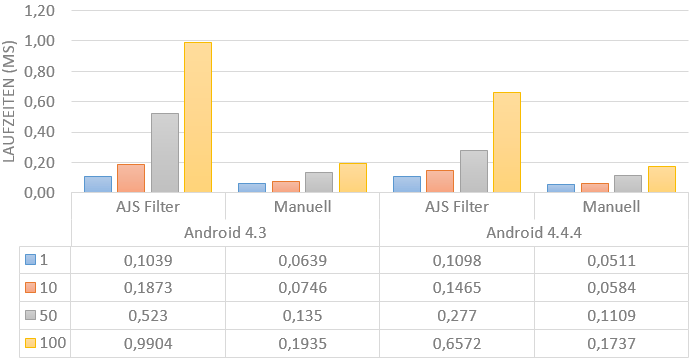
\includegraphics[scale=0.5]{Bilder/Diagramme/Filter.png}
	\caption{Daten formatieren - Laufzeitmessung}
	\label{filter-measurement}
\end{figure}
Abbildung \ref{filter-measurement} zeigt das Ergebnis dieser Analyse. Durch das Cachen der Filtermenge konnte im Mittel eine Steigerung der Performance von 173\% erreicht werden. Wenn es darum geht, komplexe Listen oder Konvertierungen durchzuführen, ist es empfehlenswert dies ohne AngularJS Filter zu implementieren. Für einfache Konvertierungen wie Datums- oder numerische Werte ist dessen Einsatz dennoch zu empfehlen, da zum einen der JavaScript-Code von unnötigem Code befreit wird und die Performance durch das AngularJS interne caching dennoch nicht beeinflusst wird. 
\begin{lstlisting}[language=JavaScript, caption={Daten formatieren, Liste manuell formatieren (Controller) }\label{formatdata-manuell-c}]
$scope.$watch('data.filter.name', filterData);
$scope.$watch('data.filter.age', filterData);

function filterData() {
	var tmp = $scope.data.items;
	tmp = $filter('filter')(tmp, $scope.data.filter.name);
	tmp = $filter('filter')(tmp, $scope.data.filter.age);
	tmp = $filter('orderBy')(tmp, 'age', true),
	$scope.data.displayList = tmp;
};
\end{lstlisting}
